\cotefile{105}
\scanpage{2}

% printed form
3 3 -- N O D E E 3 3

S E333

\handwritten{\[
\overset{\text{$Z_a$}}{\partial\longrightarrow I}
\]}

\handwritten{$\deleted{\unsure{\mathrm{ob}}}\,\unsure{\pi_0|\Pi_0}(\partial)\geq 2$\quad \deleted{\unsure{0-connexe|$\varnothing$-connexe}} \qquad \unsure{0-connexe}}

\handwritten{\[
\left\{\begin{aligned}
&\phi\longrightarrow e\\
&\partial\times S^n(N)\longrightarrow I\times S^n(N)\\
&\bigl\{+\,\text{Cônes gauches (resp. droits) sur les précédents}\\
&\text{(donne aussi }\{0\}\to\Delta^1\\
&\qquad\text{resp.}^{\mathrm{t}}\ \{1\}\to\Delta^1\text{)}
\end{aligned}\right.
\]}

\handwritten{\[
\underline{\mathrm{Hom}}(\unsure{\pi|\Pi|T|I},X)
\]}

\handwritten{\uline{Lemme} a) Si $X\longrightarrow e$ a la propriété RLP pour $\phi\longrightarrow e$ \uline{et} les $\partial\times S^n(N)\longrightarrow I\times S^n(N)$, $n\in\mathscr N$ (\unsure{partie} infinie de $N$), alors $X$ est $W_\infty$-asph.}

\handwritten{b) Si $X\longrightarrow Y$ a la RLP p.r. aux cônes gauches (resp. droits) p.r. aux morphismes précédents, alors $X$ est $W_\infty$-propre (resp. $W_\infty$-lisse).}

\handwritten{\uline{Cor} a) Si \inserted{$X\longrightarrow Y$} a la propriété RLP p.r. aux \unsure{sommes} de deux \deleted{\unsure{autres}} \inserted{(resp. \unsure{jointures|gauches})} \deleted{\unsure{entre}} catégories \deleted{\unsure{fibrées}} \uline{réunies}, \uline{finies}, et alors c'est un morphisme $W_\infty$-propre (resp. lisse) \inserted{à fibres $W_\infty$-asphériques}.}

\handwritten{b) Si $f\colon X\longrightarrow Y$ a la propriété RLP p.r. aux \inserted{\unsure{demi-cercles} (resp. \unsure{demi}) $n$\textsuperscript{es} \deleted{\unsure{triviales}} \unsure{ét.c.}} \unsure{sommes} de deux (qui s.t des $W_\infty$, \inserted{des cat finies}) alors $f$ est $W_\infty$-propre (resp. $W_\infty$-lisse). S'il a la dite propriété pour les $W_\infty$ cofibrations triviales \inserted{entre cat. finies}, alors il est $W_\infty$-parfait.}

% archive sheet number: 1
\scanpage{3}

\deleted{\unsure{Notamment|Néanmoins} on voudrait que}

\deleted{\[
\underline{\mathrm{Ar}}(C)\xrightarrow{p}C\times C
\]}

\deleted{ait des propriétés du type ``fibration'', \deleted{\unsure{ou|on}} Or

1) au sens catégorique, ce n'est ni une fibration, ni une cofibration -- et $=$ les \deleted{\unsure{projets|projections|propriétés}} composés $\underline{s}\circ p,\underline{b}\circ p\colon\underline{\mathrm{Ar}}(C)\longrightarrow C$ ne le sont pas.}

\deleted{2) De $=$, \deleted{\unsure{ni}} $p$ \deleted{\unsure{n'est}} n'est ni cohom. propre, ni coh. lisse. Peut-être au moins $\deleted{\unsure{s}}\ \underline{s}\circ p$ et $\underline{s}\circ b$ \deleted{le} sont-ils \deleted{\unsure{le}} l'un ou l'autre ? Mais ce sont plutôt les propr. de $p$ lui-$=$ qui m'importent !}

\deleted{3) Il semblerait que $p$ soit une $W_\infty$-fibration. (``fibration cohomologique'') C'est une chose à vérifier.}

\deleted{\uline{Question} Les $W_\infty$-fibrations, et la notion correspondante \inserted{(par le L.L.P)} de cofibration, \deleted{\unsure{font}} font-ils une \deleted{des} structure de Quillen sur $(Cat)$ ?}

% archive sheet number: 2
\scanpage{4}

\deleted{Ahmed}

\figure{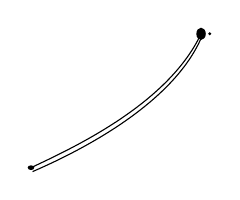
\begin{tikzpicture}[x=1cm,y=1cm]
\draw[thin] (0,0) .. controls (.60,.28) and (1.75,.83) .. (2.16,1.70);
\draw[thin] (.02,-.05) .. controls (.92,.34) and (1.88,.94) .. (2.18,1.69);
\fill (0,0) ellipse (.042 and .030);
\fill (2.16,1.70) ellipse (.060 and .078);
\fill (2.27,1.70) circle (.021);
\end{tikzpicture}}

% archive sheet number: 3
\scanpage{5}

\mspage{1}

$A$ a topos

$W\subset\mathrm{Fl}(A)$ set of arrows, \inserted{weakly} saturated i.e.

$\left\{\begin{aligned}
&\text{a) isom. are in }W\\
&\text{b) if }f=vu,\ \text{and two among}\\
&\qquad u,v,f\text{ in }W,\ \text{so the third}\\
&\text{c) if }X \mathrel{\substack{\xrightarrow{f}\\[-.6ex]\xleftarrow[g]{}}}Y\text{ with}\\
&\qquad gf=\mathrm{id}_X,\ fg\in W,\ \text{then}\\
&\qquad f,g\in W
\end{aligned}\right.$

plus other conditions we are going to list, as we need them

\deleted{\unsure{Let}} Let moreover $\deleted{C_0\subset(TC)_0}$

\[
(TC)_0\subset C_0\bigl(\subset\mathrm{Fl}(A)\bigr)
\]

(with no other assumptions for the time being). We define

% slanted
\margin{\uline{NB} $C$ stands for ``cofibrations'', $TC$ for ``trivial cofibrations'', $F$ for ``fibrations'', $TF$ for ``trivial fibrations''}

\[
\deleted{\unsure{TF\subset|TF_0}}\qquad TF\subset F\bigl(\subset\mathrm{Fl}(A)\bigr)
\]

by the right lifting property (RLP) with respect to $\deleted{(TC)_0}$ $C_0$ and $(TC)_0$ respectively, and then

\diagram{\begin{tikzcd}[ampersand replacement=\&,column sep=small,row sep=0pt]
TC \& {\subset} \& C \& {(\subset\mathrm{Fl}(A))}\\
{\cup} \& \& {\cup}\\
(TC)_0 \& {\subset} \& C_0
\end{tikzcd}}

by the \deleted{right} left lifting property \inserted{(LLP)} with respect to $F$ and $TF$ respectively. We have pairs

\diagram{\begin{tikzcd}[ampersand replacement=\&,column sep=small]
TC \arrow[rr,leftrightarrow] \& \vphantom{F}\arrow[d,dash,start anchor=north,end anchor=south] \& F\arrow[d,harpoon]\\
C\arrow[u,harpoon] \arrow[rr,leftrightarrow] \& \vphantom{F} \& TF
\end{tikzcd}}

in which each \inserted{\unsure{class|element|one}} determines the other by RLP \deleted{\unsure{ou|or}} or LLP. \deleted{Moreover} Moreover

a) $F,TF$ stable by composition, base change, direct factors

b) $C,TC$ stable by composition, cobase change, direct factors

% archive sheet number: 4
\scanpage{6}

% printed form
{\scriptsize\ttfamily\begin{tabular}{@{}l@{}}
ACCOUNT NUMBER *********,000000000 \quad DATE = \ 82.160 \qquad TIME \ =\\
JOBNAME= PREDONTA \quad NUMBER=160J0365CNU \quad CPU TOTAL = \qquad 15
\end{tabular}}

\diagram{{\scriptsize\ttfamily\begin{tabular}{@{}l@{}}
********************************************************************\\
*~~~~~~~~~*~~~~~~~~~~~~~~~*\\
*~S~T~E~P~*~~~~T~I~M~E~~~~*~~~~~N~~~~U~~~~M~~~~B~~~~E~~~~R~~~~~O~~F\\
*~~~~~~~~~*~~~~~~~~~~~~~~~*\\
********************************************************************\\
*~~*~~~~~~*~~~~~~~*~~~~~~~*~~~~~~*~~~~~~*~~~~~~*~~~~~~*~~~~~~*\\
*NO*~CORE~*~~TIO~~*~TCPU~~*~3330~*3330-1*~3340~*~3350~*~2250~*T/7TRK\\
*~~*~~~~~~*~~~~~~~*~~~~~~~*~~~~~~*~~~~~~*~~~~~~*~~~~~~*~~~~~~*\\
********************************************************************\\
*~~*~~~~~~*~~~~~~~*~~~~~~~*~~~~~~*~~~~~~*~~~~~~*~~~~~~*~~~~~~*\\
*~1*~~~84~*~~~~~18*~~~~~14*~~~~~1*~~~~~3*~~~~~0*~~~~~0*~~~~~0*~~~~~0\\
*~~*~~~~~~*~~~~~~~*~~~~~~~*~~~~~~*~~~~~~*~~~~~~*~~~~~~*~~~~~~*\\
********************************************************************\\
*~~~~~~~~~*~~~~~~~*~~~~~~~*~~~~~~*~~~~~~*~~~~~~*~~~~~~*~~~~~~*\\
*~TOTALS~~*~~~~~18*~~~~~14*~~~~~1*~~~~~3*~~~~~0*~~~~~0*~~~~~0*~~~~~0\\
*~~~~~~~~~*~~~~~~~*~~~~~~~*~~~~~~*~~~~~~*~~~~~~*~~~~~~*~~~~~~*\\
********************************************************************
\end{tabular}}}

\diagram{{\scriptsize\ttfamily\begin{tabular}{@{}l@{}}
********************************************************************\\
*~~~~~~~~~~~~~~~~~~~~~~~~~~~~~~~~~~~~*~~~~~~~~~~~~~~~*\\
*~~~~~~~~S~~~~~~T~~~~~~E~~~~~~P~~~~~~*~~~~PAGING~~~~~*~~~~S~~~W~~~A\\
*~~~~~~~~~~~~~~~~~~~~~~~~~~~~~~~~~~~~*~~~~~~~~~~~~~~~*\\
********************************************************************\\
*~~*~~~~~~~~*~~~~~~~~*~~~~~~~*~~~~~~~*~~~~~~~*~~~~~~~*~~~*~~~~~~~*\\
*NO*~NAME~~~*~~P~G~M~*~C.C.U~*~SRB~~~*~~IN~~~*~~OUT~~*~N~*~P.OUT~*~\unsure{F|P}\\
*~~*~~~~~~~~*~~~~~~~~*~~~~~~~*~~~~~~~*~~~~~~~*~~~~~~~*~~~*~~~~~~~*\\
********************************************************************\\
*~~*~~~~~~~~*~~~~~~~~*~~~~~~~*~~~~~~~*~~~~~~~*~~~~~~~*~~~*~~~~~~~*\\
*~1*CSSBATCH*CRBATCH~*~~~~163*~~~~~~1*~~~~~~0*~~~~~~0*~~0*~~~~~~0*\\
*~~*~~~~~~~~*~~~~~~~~*~~~~~~~*~~~~~~~*~~~~~~~*~~~~~~~*~~~*~~~~~~~*\\
********************************************************************\\
*~~~~~~~~~~~~~~~~~~~~*~~~~~~~*~~~~~~~*~~~~~~~*~~~~~~~*~~~*~~~~~~~*\\
*~~T~~O~~T~~A~~L~~S~~*~~~~400*~~~~~~1*~~~~~~0*~~~~~~0*~~0*~~~~~~0*\\
*~~~~~~~~~~~~~~~~~~~~*~~~~~~~*~~~~~~~*~~~~~~~*~~~~~~~*~~~*~~~~~~~*\\
********************************************************************
\end{tabular}}}

{\scriptsize\ttfamily\begin{tabular}{@{}l@{}}
~~RESOURCES ESTIMATED~~(~SYSOUT~=~0120000~~EXCP~=~~~~1000~~TIME~=\\
~~RESOURCES USED~~~~~~~(~SYSOUT~=~0001271~~EXCP~=~~~~~~~4~~TIME~=\\
\$HASP399 ENDED
\end{tabular}}

% archive sheet number: 5
\scanpage{7}

\mspage{2}

\[
\begin{aligned}
\text{c) }\text{\deleted{$X\longrightarrow Y$ is $\in W$}}\quad TC&=C\cap\widetilde W\\
TF&=F\cap\widetilde W
\end{aligned}
\]

where

\[
\begin{array}{ll}
\widetilde W&\subset\mathrm{Fl}(A)\\
\Vert&\\
\multicolumn{2}{l}{\{f=pi\mid p\in TF,\ i\in TC\}}
\end{array}
\]

\uline{NB} These facts do only make use of the existence of \deleted{\unsure{fini|fin.}} amalgamated sums and fibered products in $A$ (not of the fact that $A$ is a topos, -- and for the time being $W$ has not been used). We used only the symmetric relationship between \deleted{\unsure{bet}} $(TC,F)$, and $(C,TF)$, \deleted{not} plus $TC\subset C$ ($\Longleftrightarrow TF\subset F$), not the way they were obtained by some \inserted{pair} $(TC)_0\subset C_0$.

d) \deleted{Assume $TC$, If $i\in C$, $f\in$} \inserted{Consider \deleted{\unsure{let|bet|but}}, for any}

\[
\begin{array}{cc}
i\colon A\longrightarrow B&f\colon X\longrightarrow Y\\
\deleted{i\in C}&\deleted{f\in F}
\end{array}
\]

\deleted{Consider}

\[
\underline{\mathrm{Hom}}(B,X)\xrightarrow{\underline{\alpha}(i,f)}
\underline{\mathrm{Hom}}(i,f)\overset{\mathrm{def}}=
\underline{\mathrm{Hom}}(B,Y)\mathop{\times}_{\underline{\mathrm{Hom}}(A,Y)}\underline{\mathrm{Hom}}(A,\unsure{X})
\]

\deleted{Then $\alpha(i,f)\in$} Then we have the following \deleted{equivalences}

(i) $C,TC$ stable by cartesian products $? \times Z$

$\Updownarrow$ (ii) $TF$, $\deleted{\unsure{T}}\,F$ stable by $\underline{\mathrm{Hom}}(Z,?)$

$\Updownarrow$ (iii) If $i\in C$, $f\in F$, then $\alpha(i,f)\in F$, and if moreover $i\in TC$ or $f\unsure{\in|\theta}TF$, then $\alpha(i,f)\in TF$.

% slanted
\margin{under suitable assumptions}

% archive sheet number: 6
\scanpage{8}

% printed form
{\scriptsize\ttfamily\begin{tabular}{@{}l@{}}
9.14.21 \qquad SYSTEM~~370/081 E333 \quad VS2 03.8G\\
~~~~~~~RATE~~~=~0,~1
\end{tabular}}

\diagram{{\scriptsize\ttfamily\begin{tabular}{@{}l@{}}
****************************************************\\
~~~~~~~~~~~~~~~~~~~~~~~~~~~~*~~~~~~~~~~~~~~*~~~~~~~*\\
~~~~E~~~~X~~~~C~~~~P~~~~S~~~*~~~~~BYTES~~~~*~~~~~~~*\\
~~~~~~~~~~~~~~~~~~~~~~~~~~~~*~~~~~~~~~~~~~~*~~~~~~~*\\
****************************************************\\
*~~~~~~*~~~~~~*~~~~~~*~~~~~~*~~~~~~*~~~~~~~*~~~~~~~*\\
*T/8-16*T/6250*~SPOOL*~VIO~~*SYSIN~*SYSOUT~*~~C.U~~*\\
*~~~~~~*~~~~~~*~~~~~~*~~~~~~*~~~~~~*~~~~~~~*~~~~~~~*\\
****************************************************\\
*~~~~~~*~~~~~~*~~~~~~*~~~~~~*~~~~~~*~~~~~~~*~~~~~~~*\\
*~~~~~0*~~~~~0*~~~~~1*~~~~~0*~~~526*0001271*~~~~163*\\
*~~~~~~*~~~~~~*~~~~~~*~~~~~~*~~~~~~*~~~~~~~*~~~~~~~*\\
****************************************************\\
*~~~~~~*~~~~~~*~~~~~~*~~~~~~*~~~~~~*~~~~~~~*~~~~~~~*\\
*~~~~~0*~~~~~0*~~~~~1*~~~~~0*~~~526*0001271*~~~~163*\\
*~~~~~~*~~~~~~*~~~~~~*~~~~~~*~~~~~~*~~~~~~~*~~~~~~~*\\
****************************************************
\end{tabular}}}

\diagram{{\scriptsize\ttfamily\begin{tabular}{@{}l@{}}
****************************************************\\
~~~~~*~~~~~~~~~~~~~~~*~~~~~~~~~~~*~~~~~~~~~~~*~~~~~*\\
~~P~~*~~~V~~~I~~~O~~~*~~~CORE~~~~*~S~E~T~U~P~*TIME~*\\
~~~~~*~~~~~~~~~~~~~~~*~~~~~~~~~~~*~~~~~~~~~~~*~~~~~*\\
****************************************************\\
~~~~~*~~~~~~~*~~~~~~~*~~~~~*~~~~~*~~*~~*~~*~~*~~~~~*\\
\unsure{P}.IN~*~P.IN~~*~P.OUT~*~TOT~*~TOP~*DU*DM*TU*TM*ELAPS*\\
~~~~~*~~~~~~~*~~~~~~~*~~~~~*~~~~~*~~*~~*~~*~~*~~~~~*\\
****************************************************\\
~~~~~*~~~~~~~*~~~~~~~*~~~~~*~~~~~*~~*~~*~~*~~*~~~~~*\\
~~~~0*~~~~~~0*~~~~~~0*~5360*~~244*~0*~0*~0*~0*~~~~2*\\
~~~~~*~~~~~~~*~~~~~~~*~~~~~*~~~~~*~~*~~*~~*~~*~~~~~*\\
****************************************************\\
~~~~~*~~~~~~~*~~~~~~~*~~~~~*~~~~~*~~*~~*~~*~~*~~~~~*\\
~~~~0*~~~~~~0*~~~~~~0*~~~~~*~~~~~*~~*~0*~~*~0*~~~~2*\\
~~~~~*~~~~~~~*~~~~~~~*~~~~~*~~~~~*~~*~~*~~*~~*~~~~~*\\
****************************************************
\end{tabular}}}

{\scriptsize\ttfamily\begin{tabular}{@{}l@{}}
~~6~~REGION~=~~~150K~)~~GIVING~CLASS/PRIO~~=~Q/~0\\
~~1~~REGION~=~~~~84K~)~~GIVING~CLASS/PRIO~~=~A/14
\end{tabular}}

% archive sheet number: 7
\scanpage{10}

\mspage{3}

\uline{Proof} $(i)\Longrightarrow(ii)$ Assume $(i)$, let $f\colon X\longrightarrow Y$, $f\in F$, prove $\deleted{\underline{\mathrm{Hom}}(T,f):}$

\[
\bigl(\underline{\mathrm{Hom}}(T,f)\colon\underline{\mathrm{Hom}}(T,X)\longrightarrow\underline{\mathrm{Hom}}(T,Y)\bigr)\in F
\]

i.e. \deleted{\unsure{L|R}}RLP with respect to any $i\colon A\longrightarrow B$ \inserted{in $TC$} -- this amounts to RLP of $f$ with respect to $i\times\mathrm{id}_T\colon A\times T\longrightarrow B\times T$, OK as this is \inserted{still} in $TC$. Same for $f\in TC$, using stability of $C$ under $\times T$.

$(ii)\Longrightarrow(i)$ Assume $(ii)$, let $i\colon A\longrightarrow B$, \deleted{prove} \inserted{in $C$}, prove $i\times T\colon A\times T\longrightarrow B\times T$ is still in $C$, i.e. has \deleted{right} LLP with respect to any $f\in TF$, but this amounts to $i$ having the same with respect to $\mathrm{Hom}(T,f)$, which is still in $TF$ by assumption OK.

\deleted{$\unsure{(i)}\ (i)\unsure{+}(ii)\Longrightarrow(iii)$} \uline{NB} The equivalence $(i)\Leftrightarrow(ii)$ could be further axiomatized, as a relation between $\unsure{\Phi|\mathscr L}^{*}_{\deleted{*}},\Phi^{\deleted{*}}_{*}$ associated by LLP and RLP, when we have two functors $\otimes,\underline{\mathrm{Hom}}$ tied by the Cartan relation

\[
\mathrm{Hom}(A\otimes T,X)\simeq\mathrm{Hom}(A,\underline{\mathrm{Hom}}(T,X)).
\]

\deleted{$(i)\,(ii)\longrightarrow\unsure{(i)|(iii)}$}

Moreover, when we have stability of $\Phi_{\deleted{*}}^{*}$ under $\deleted{\unsure{\otimes}\ T\otimes ?}\inserted{?\otimes T}$ \inserted{(when $\Phi^{*}$ is either $C$ or $TC$)} or equivalently of $\Phi^{*}_{*}$ under $\underline{\mathrm{Hom}}(T,?)$, then for $i\colon A\longrightarrow B$ in $\Phi^{*}$, $f\colon X\longrightarrow Y$ in $\Phi$, we'll have that

\[
\deleted{\underline{\mathrm{Hom}}(i,f)}\ \inserted{\underline{\alpha}(i,f)}\ \deleted{\unsure{\alpha(i,f)}}\colon
\underline{\mathrm{Hom}}(B,X)\longrightarrow\underline{\mathrm{Hom}}(i,f)
\quad\underline{\text{is in }TF}\ \text{\inserted{(is in $\Phi_{*}$ ?)}}.
\]

Indeed, this means it has RLP with respect to any $\unsure{j'|i'}\colon A'\longrightarrow B'$ in $C$ \inserted{[$\Phi^{*}$]}, i.e.

\[
\mathrm{Hom}(B',\underline{\mathrm{Hom}}(B,X))\longrightarrow
\mathrm{Hom}\bigl(\unsure{j'|i'|j},\deleted{\alpha(i,f)}\inserted{\unsure{\mathrm{Hom}}(\deleted{\unsure{\alpha}}\unsure{i'|i},f)}\bigr)
\]

is surjective. But \deleted{the first hand \unsure{expression|member}} \inserted{this can be viewed as}

\[
\begin{aligned}
&\deleted{\mathrm{Hom}(B'\otimes B,X)}\\
&\mathrm{Hom}(B'\otimes B,X)\longrightarrow\mathrm{Hom}(\deleted{i'\otimes i}\deleted{\unsure{\boxtimes(i',i)}}\inserted{i'\boxtimes i},f)
\end{aligned}
\]

% slanted
\margin{check language more carefully}

where

\[
\begin{aligned}
&\deleted{i'\otimes i\colon A'\otimes A\longrightarrow B'\otimes B}\\
&i'\boxtimes i\quad \deleted{\unsure{\alpha(i,i')}}\deleted{i'\boxtimes i}\quad A'\otimes B\amalg_{A'\otimes A}B'\otimes A\longrightarrow B'\otimes B
\end{aligned}
\]

\deleted{and} Thus we have to check that if $i,i'\in\Phi^{*}$, then $i\boxtimes i'$ is in $\Phi^{*}$ [OK if $\Phi^{*}$ are monomorphisms, say, and $\otimes=$ cartesian product]

% slanted
\margin{and conversely}

Coming back to case of $(C,TF),(TC,F)$, this shows that if $i\in C$, $f\in TF$, then $\deleted{\unsure{\mathrm{Hom}}}\alpha(i,f)$ is in $TF$, -- and if $i$ is in $TC$ and $f$ in $F$, then $\alpha(i,f)$ is in $F$,

% archive sheet number: 9
\scanpage{11}

% printed form
{\scriptsize\ttfamily STMT NO. MESSAGE\\
-\\
~~~~4~~~~~IEF653I SUBSTITUTION JCL - PGM=CRBATCH,REGION=100K,PARM=}

{\scriptsize\ttfamily \$HASP373 STARTED - INIT 10 - CLASS Q - SYS E333\\
IEF236I ALLOC. FOR PREDONTA CSSBATCH\\
IEF237I 581~~ALLOCATED TO STEPLIB\\
IEF237I 2C9~~ALLOCATED TO SYS00052\\
IEF237I VIO~~ALLOCATED TO SYSUT1\\
IEF237I JES2 ALLOCATED TO SYSUDUMP\\
IEF237I 59F~~ALLOCATED TO CRJIF\\
IEF237I JES2 ALLOCATED TO SYSIN\\
IEF237I 59F~~ALLOCATED TO SYS00002\\
IEF237I 59F~~ALLOCATED TO SYS00001\\
IEF285I~~~CRAY1.PREDONT.CSS.D82160.T091420.R70 \quad CATALOGED\\
IEF285I~~~VOL SER NOS= CRAY11.}

{\scriptsize\ttfamily CSS2060 - JOB QUEUED FOR TRANSFER\\
IEF142I PREDONTA CSSBATCH - STEP WAS EXECUTED - COND CODE 0000\\
IEF285I~~~CISI.PROD.CSSBATCH.V1.YY01 \quad KEPT\\
IEF285I~~~VOL SER NOS= MVS104.\\
IEF285I~~~SYSCTLG.VSAC015 \quad KEPT\\
IEF285I~~~VOL SER NOS= SAC015.\\
IEF285I~~~SYS82160.T091418.RA000.PREDONTA.SYSUT1 \quad DELETED\\
IEF285I~~~JES2.JOB00365.\unsure{SO0102|S00102} \quad SYSOUT\\
IEF285I~~~SYS1.CR.JIF \quad KEPT\\
IEF285I~~~VOL SER NOS= CRAY11.\\
IEF285I~~~JES2.JOB00365.SI0101 \quad SYSIN\\
IEF285I~~~SYSCTLG.VCRAY11 \quad KEPT\\
IEF285I~~~VOL SER NOS= CRAY11.}

{\scriptsize\ttfamily IEF373I STEP /CSSBATCH/ START 82160.0914\\
IEF374I STEP /CSSBATCH/ STOP~~82160.0914 CPU~~0MIN 00.14SEC SRB~~0MIN 00.01SEC VIRT~~~84K SYS~~~244K\\
IEF375I~~JOB /PREDONTA/ START 82160.0914\\
IEF376I~~JOB /PREDONTA/ STOP~~82160.0914 CPU~~0MIN 00.14SEC SRB~~0MIN 00.01SEC}

% archive sheet number: 10
\scanpage{12}

\mspage{4}

provided \deleted{we} check that if $i,i'\in TC$, \inserted{(resp. in $C$?)} then $\deleted{\unsure{\in|C}}i'\boxtimes i$ is in $TC$ \inserted{(resp. in $C$?)}. But \inserted{if} this is to occur if we assume only \uline{one} of the two arrows $i,i'$ in $TC$, the other being in $C$, then we get even that $i\in TC,f\in F\Longrightarrow\alpha(i,f)\in TF$ and $i\in C,f\in F\Rightarrow\alpha(i,f)\in F$.

We just need formally

\[
\alpha(i',\underline{\alpha}(i,f))\simeq\alpha(i'\boxtimes i,f)
\]

\uline{To sum up} we get equivalences

\[
\begin{aligned}
\deleted{C\ \text{stable by }?\otimes T}\ C\otimes T\subset C&\Longleftrightarrow TF\ \text{stable by }\underline{\mathrm{Hom}}(T,?)\ ;\\
\deleted{\unsure{TC}\ \text{stable by }?\otimes T}\ TC\otimes T\subset TC&\Longleftrightarrow F\ \text{stable by }\underline{\mathrm{Hom}}(T,?)\\
\deleted{C\ \text{stable by }i'\boxtimes i^{\unsure{*|'}}}\ C\boxtimes C\subset C&\Longleftrightarrow(i\in C,f\in TF\Longrightarrow\underline{\alpha}(i,f)\in TF)\\
\deleted{\unsure{i\in C,\ i'\in C}}\ \deleted{\unsure{TC\boxtimes TC|C\boxtimes TC}}\ TC\boxtimes TC\subset TC&\Longleftrightarrow(i\in TC,f\in F\Longrightarrow\underline{\alpha}(i,f)\in \deleted{\unsure{T}}F)\\
TC\boxtimes C\subset TC&\Longleftrightarrow(i\in C,f\in F\Longrightarrow\underline{\alpha}(i,f)\in F)
\end{aligned}
\]

\margin{\deleted{\unsure{symm.} \unsure{possibility|property}}}

\uline{Example} \inserted{$A$ a topos} $\otimes={}$ cartesian product, $\underline{\mathrm{Hom}}$ the usual \inserted{(\unsure{my notation|my writing|inner notation|inner writing})} Hom,

\deleted{$A$ a topos} $C=\mathrm{mono}$, $(TC)_0={}$ monomorphisms of the type

\[
\deleted{\unsure{I\ (A_0\times B_0)}}\ \inserted{(B_0\times e)\cup}\ (A_0\times I)\overset{i}{\subset}\deleted{\unsure{I}}\times B_0\times I,
\]

where $\deleted{B}A_0\xrightarrow{i_0}B_0$ any mono $I$ any \uline{$W$-aspheric object} over $e_A$ endowed with section $e$.

\margin{given bunch of $I$'s with given sections}

$C$ stable by $? \times T$: trivial, hence $F$ stable by $\underline{\mathrm{Hom}}(T,?)$

$(TC)_0$ stable by $?\times T$ (replace $i_0$ by $i_0\times\mathrm{id}_T$) hence $F$ stable by $\underline{\mathrm{Hom}}(T,?)$, hence $TC$ stable by $?\times T$

\deleted{$C$ stable by $i'\boxtimes i$: trivial}

$C\boxtimes C\subset C$: trivial

To check $TC\boxtimes C\subset TC,\ C\boxtimes TC\subset TC$. Consider $i$ defined by $i_0\colon A_0\longrightarrow B_0,I,e$ \inserted{(i.e. $i=h(i_0,A_0,B_0)$)} and $i'\colon A'\longrightarrow B'$, consider the diagram

\diagram{\begin{tikzcd}[ampersand replacement=\&]
A^{\unsure{'}}\times A^{\deleted{\unsure{'}}}\arrow[r,hook]\arrow[d,hook] \& B'\times\deleted{\unsure{B}}A\arrow[d,hook]\\
\deleted{\unsure{B|A}}A'\times\deleted{A}B\arrow[r,hook] \& B'\times\deleted{\unsure{A}}B^{\deleted{\unsure{'}}}=B'_{\deleted{\unsure{0}}}\times B_0\times I
\end{tikzcd}}

% archive sheet number: 11
\scanpage{13}

% printed form
{\scriptsize\ttfamily 1~~~~//PREDONTA JOB '*********,000000000','\hspace{7em}',\hfill JOB 0365\\
~~~~~// MSGLEVEL=(1,1)}

{\scriptsize\ttfamily 2~~~~//~~~~~~~~~EXEC CSSBATCH \hfill 00000040\\
3~~~~XXCSSBATCH PROC REG=100K,P='' \hfill 00010000\\
4~~~~XXCSSBATCH EXEC PGM=CRBATCH,REGION=\&REG,PARM=\&P \hfill 00020000\\
5~~~~XXSTEPLIB~~DD DSN=CISI.PROD.CSSBATCH.V1.YY01,DISP=SHR \hfill 00030003\\
6~~~~XXSYSUT1~~~DD DSN=\&\&SYSUT1,UNIT=\unsure{SYSTSO|SYSTS0},SPACE=(TRK,30),DISP=(NEW,DELETE) \hfill 00031006\\
7~~~~XXSYSUDUMP DD SYSOUT=* \hfill 00040000\\
8~~~~XXCRJIF~~~~DD DSN=SYS1.CR.JIF,DISP=SHR \hfill 00050000\\
9~~~~XXSYSIN~~~~DD DDNAME=CRAYIN \hfill 00060000\\
10~~~//CRAYIN~~~DD * \hfill 00000050\\
~~~~~// \hfill 00000160}

% archive sheet number: 12
\scanpage{14}

\mspage{5}

\diagram{\begin{tikzcd}[ampersand replacement=\&,column sep=large,row sep=huge]
((A'\times B_0)\times e)\cup(A'\times A_0\times I)\arrow[r]\arrow[d,"{\big\}h(i_0\times\mathrm{id}_{A'},I,e)}"] \& ((\deleted{\unsure{A}}B'\times B_0)\times e)\cup((B'\times A_0)\deleted{\unsure{\times}}\times\deleted{\unsure{A}}I)\arrow[d,"{h(i_0\times\mathrm{id}_{\unsure{B'}},I,e)\big\{}"']\\
\underbrace{(A'\times B_0)}\times\deleted{\unsure{B}}I\arrow[r,hook] \& B'\times B_0\times\deleted{\unsure{B}}I
\end{tikzcd}}

\deleted{$A'\times B_0\quad\unsure{A'\ h(i|A'\boxtimes h(i}$}

On trouve $i'\boxtimes(i=h(i_0,I,e))=h(i'\boxtimes i_0,I,e)$ et la formule symétrique, donc on gagne.

\margin{\uline{vérifier avec soin}}

\uline{We do not know yet} M1 (factorisation of any $f$ as $pi$, with either $i\in C,p\in TF$, or $i\in TC,p\in F$), nor M5 (saturation of $\widetilde W$ -- indeed we need only check a) b) to have a closed model category). The factorisation $f=pi$ is the usual argument for constructing \unsure{injectives}, using \unsure{reasonable|reasonably} properties of existence of \inserted{small} generating set of $A$, and of filtering direct limits.

The lifting property may again be axiomatized in terms of $\unsure{\Phi|\mathscr L}^{*}_{\deleted{*}},\Phi_{*}$, in a topos or a more general category -- I'll not for the moment work out these general formulations, and \deleted{\unsure{be content|to content}} I'll assume this factorizability \deleted{\unsure{of|any $f$}} in the two ways.

% slanted
\margin{\uline{to work out}}

We now want to identify $\widetilde W$, and check condition b) of saturation. We want even prove $\widetilde W=W$ -- now it becomes essential to \deleted{\unsure{exp}} make clear how the definition of $(TC)_0$ \uline{depends} on $W$, taking as ``bunch'' of \deleted{intervals} all intervals $I$ which are $W$-aspheric over $e$. But this may make a difficulty for factorisation,

% archive sheet number: 13
\scanpage{15}

% printed form
{\scriptsize\ttfamily J E S 2~~J O B~~L O G~~--~~S Y S T E M~~E 3 3 3~~--~~N O D E~~E 3 3}

{\scriptsize\ttfamily 09.14.18 J0365CNU~~\$ J0365*PREDONTA STARTED - INIT 10 - CLASS Q - SYS E333\\
09.14.19 J0365CNU~~DSN CISI.PROD.CSSBATCH.V1.YY01\\
09.14.21 J0365CNU~~CSS2060 - JOB QUEUED FOR TRANSFER\\
09.14.21 J0365CNU~~SMF RECORD 153-1 (CLOSE) WRITTEN\\
09.14.22 J0365CNU~~\$ J0365*PREDONTA ENDED}

{\scriptsize\ttfamily ------ JES2 JOB STATISTICS ------\\[1em]
09 JUN 82 JOB EXECUTION DATE\\[1em]
~~~~~~~16 CARDS READ\\[1em]
~~~~~~100 SYSOUT PRINT RECORDS\\[1em]
~~~~~~~~0 SYSOUT PUNCH RECORDS\\[1em]
~~~~~0.06 MINUTES EXECUTION TIME}

% archive sheet number: 14
\scanpage{16}

\mspage{6}

because this bunch is not ``small'', we'll therefore take \uline{some} such bunch, and see what we need on it to be able to conclude $\widetilde W=W$.

$\widetilde W\overset{?}{\subset}W$. We are reduced to proving $TC\subset W,TF\subset W$. As $TF$ is defined in terms of $C={}$ monomorphisms, the inclusion

\[\boxed{TF\subset W}\]

may be taken as an axiom on $W$. But in case We get an \inserted{separating} interval -- $I$ which is $TF$ over $e$ i.e. an injective object, \deleted{we may \unsure{then|take}} this inclusion is equivalent with

\[\boxed{\begin{aligned}
(I\longrightarrow e)\in UW\quad&\text{i.e.}\quad(I\times X\longrightarrow X)\unsure{\in W|\text{is such}|\text{is in }W}\\[-2pt]
&\text{for any }X
\end{aligned}}\]

% slanted
\margin{\deleted{\unsure{strictly|strict}}\inserted{strongly} modelizing topos: if there is such an $I$, namely $\{0,1\}_A$ can be \unsure{embedded|imbedded} in \unsure{injective} $\Longleftrightarrow$ but this is always true, because the \unsure{Lawvere|lower} object is injective!!!}

Thus, the axiom is really

\[
\text{\textcircled{1}}\quad\boxed{(\overset{\text{\inserted{Lawvere element}}}{L}_A\longrightarrow e)\in UW}
\]

% slanted
\margin{or equivalently: $\exists$ \uline{separating interval $\underline I$} with $(I\longrightarrow e)\in UW$}

this implies that any $\underline L$-homotopism is in $W$. But for \uuline{any} separating interval $\underline I$, it is clear that $f\in TF\Longrightarrow f$ \deleted{\unsure{as}}is a $I$-homotopism.

Next we got to prove $TC\subset W$. We need first of all $(TC)_0\subset W$.

\diagram{\begin{tikzcd}[ampersand replacement=\&]
\deleted{\unsure{(B_0\times e)}}\,A_0\times\{\deleted{\unsure{I}}e\}\arrow[r,hook]\arrow[d,hook,"W"'] \& B_0\times\{e\}\arrow[d,hook,"\Rightarrow W"]\arrow[dr,"W"] \& \\
A_0\times I\arrow[r,hook] \& A\arrow[r,hook] \& B=B_0\times I
\end{tikzcd}}

We need for this

if $S\overset{i}{\lhook\joinrel\longrightarrow}T$ mono, and $S\overset{g}{\lhook\joinrel\longrightarrow}S'$ mono $\in W$ then in

\diagram{\begin{tikzcd}[ampersand replacement=\&]
S\arrow[r,hook,"i"]\arrow[d,hook,"g"'] \& T\arrow[d,hook,"f"]\\
S'\arrow[r,hook,"i'"] \& S'\amalg_S T=T'
\end{tikzcd}}

$f\in W$

and

% archive sheet number: 15
\scanpage{17}

% printed form
{\scriptsize\ttfamily\begin{tabular}{@{}l@{}}
*******************************************************************************\\
*JESNEWS~DU~13/05/1982~C68~CADARACHE~~~~~~~~~~~~~~~~~~~~~~~~~~~~~~~~~~~~~~~~~~*\\
*******************************************************************************\\
*~~~~~~2.~LA~NUMEROTATION~DES~JOBS~SUR~C68~SERA~DORENAVANT,LEGEREMENT~~~~~~~~~*\\
*~~DIFFERENTE:~~FORME~NOUVELLE~...~~JXXXXC68~~~~~~~~~~~~~~~~~~~~~~~~~~~~~~~~~~*\\
*~~~~~~~~~~~~~~~FORME~ANCIENNE~...~~JOBXXXXC~~~~~~~~~~~~~~~~~~~~~~~~~~~~~~~~~~*\\
*~~~~~~~~~~~~~~~~~~~~~~~~~~~~~~~~~~~~~~~~~~~~~~~~~~~~~~~~~~~~~~~~~~~~~~~~~~~~~*\\
*~~~NOTA~BENE~~:~~~LA~FORME~ANCIENNE~SUBSISTERA~SUR~LES~AUTRES~NOEUDS~D~EXECU~*\\
*~~~~~~~~~~~~~~~~~~TION~DU~RESEAU~,JUSQU~A~CE~QU~ILS~PASSENT~A~CETTE~NOUVELLE~*\\
*~~~~~~~~~~~~~~~~~~VERSION~DE~JES2~~~~~~~~~~~~~~~~~~~~~~~~~~~~~~~~~~~~~~~~~~~~*\\
*******************************************************************************\\
*~UTILISATEURS~C68~CADARACHE~~~~~~~~~~~~~~~~~~~~~~~~~~~~~~~~~~~~~~~~~~~~~~~~~~*\\
*~~~~~~~~~~~~~~~~~~~~~~~~~~~~~~~~~~~~~~~~~~~~~~~~~~~~~~~~~~~~~~~~~~~~~~~~~~~~~*\\
*~MISE~EN~SERVICE~D'UN~NOUVEAU~VOLUME~GAF~:~~~CAD520~SAUVEGARDE~HEBDO~~~~~~~~~*\\
*~A~PARTIR~DU~MERCREDI~28~AVRIL~1982.~~~~~~~~~~~~~~~~~~~~~~~~~~~~~~~~~~~~~~~~~*\\
*~~~~~~~~~~~~~~~~~~~~~~~~~~~~~~~~~~~~~~~~~~~~~~~~~~~~~~~~~~~~~~~~~~~~~~~~~~~~~*\\
*******************************************************************************\\
*~~~~~~~~~~~~~~~~~~~~~~~~~~~~~~~~~~~~~~~~~~~~~~~~~~~~~~~~~~~~~~~~~~~~~~~~~~~~~*\\
*~~FORTRAN~VS~~:~~~~~~~~~~~~~~~~~~~~~~~~~~~~~~~~~~~~~~~~~~~~~~~~~~~~~~~~~~~~~~*\\
*~~-------------~~~~~~~~~~~~~~~~~~~~~~~~~~~~~~~~~~~~~~~~~~~~~~~~~~~~~~~~~~~~~~*\\
*~~~~~~~~~~~~~~~~~~~~~~~~~~~~~~~~~~~~~~~~~~~~~~~~~~~~~~~~~~~~~~~~~~~~~~~~~~~~~*\\
*~~~~~~~~MISE~EN~SERVICE~A~PARTIR~DU~13/05/1982~DU~~F~O~R~T~R~A~N~-~V~S~.~~~~~*\\
*~~~~~~~~~~~~~~~~~~~~~~~~~~~~~~~~~~~~~~~~~~~~~~~~~~~~~~~~~~~~~~~~~~~~~~~~~~~~~*\\
*~~~~~~~~ATTENTION~~TAILLE~MINIMUN~POUR~LA~COMPILATION~~920K~~~~~~~~~~~~~~~~~~*\\
*~~~~~~~~~~~~~~~~~~~~~~~~~~~~~~~~~~~~~~~~~~~~~~~~~~~~~~~~~~~~~~~~~~~~~~~~~~~~~*\\
*~~~~~~~~PROCEDURES~STANDARD~:~~~~~~~~~~~~~~~~~~~~~~~~~~~~~~~~~~~~~~~~~~~~~~~~*\\
*~~~~~~~~~~~~~~~~~~~~~~~~~~~~~~~~~~~~~~~~~~~~~~~~~~~~~~~~~~~~~~~~~~~~~~~~~~~~~*\\
*~~~~~~~~FORTVC~~CL~~CLG~.........~~~~~~~~~~~~~~~~~~~~~~~~~~~~~~~~~~~~~~~~~~~~*\\
*~~~~~~~~~~~~~~~~~~~~~~~~~~~~~~~~~~~~~~~~~~~~~~~~~~~~~~~~~~~~~~~~~~~~~~~~~~~~~*\\
*~~~~~~~~~~~~~~~~~~~~~~~~~~~~~~~~~~~~~~~~~~~~~~~~~~~~~~~~~~~~~~~~~~~~~~~~~~~~~*\\
*~~~~~~~~~~~~~~~~~~~~~~~~~~~~~~~~~~~~~~~~~~~~~~~~~~~~~~~~~~~~~~~~~~~~~~~~~~~~~*\\
*~~~~~~~~~~~~~~~~~~~~~~~~~~~~~~~~~~~~~~~~~~~~~~~~~~~~~~~~~~~~~~~~~~~~~~~~~~~~~*
\end{tabular}}

{\scriptsize\ttfamily\begin{tabular}{@{}l@{}}
******************************************************************\\
*~~~~~~~~~~~~~~~~~~~~~~~~~~~~~~~~~~~~~~~~~~~~~~~~~~~~~~~~~~~~~~~~*\\
*~~~~~~~~~~~~~~~~~~-~~J~E~S~N~E~W~S~~~F~R~1~~-~~~~~~LE~01/06/82~~*\\
*~~~~~~~~~~~~~~~~~~~~~~~~~~~~~~~~~~~~~~~~~~~~~~~~~~~~~~~~~~~~~~~~*\\
*----------------------------------------------------------------*\\
*~~~~~~~~~~~~~~~~~~~~~~~~~~~~~~~~~~~~~~~~~~~~~~~~~~~~~~~~~~~~~~~~*\\
*~-MISE~EN~SERVICE~DE~HSM~SUR~IBM~SACLAY~~~~~~~~~~~~~~~~~~~~~~~~~*\\
*~--------------------------------------~~~~~~~~~~~~~~~~~~~~~~~~~*\\
*~-HSM~EST~EN~FONCTION~ET~GERE~LES~VOLUMES~DITS~'SANS~SAUVEGARDE'*\\
*~~~~~~~~~~~~~~~~~~~~~~~~~~~~~~~~~~~~~~~~~~~~~~~~~~~~~~~~~~~~~~~~*\\
*----------------------------------------------------------------*\\
*~~~~~~~~~~~~~~~~~~~~~~~~~~~~~~~~~~~~~~~~~~~~~~~~~~~~~~~~~~~~~~~~*\\
*~~NOTE~AUX~UTILISATEURS~NOS~:~~~~~~~~~~~~~~~~~~~~~~~~~~~~~~~~~~~*\\
*~~---------------------------~~~~~~~~~~~~~~~~~~~~~~~~~~~~~~~~~~~*\\
*~~~~~~~LES~UTILISATEURS~QUI~SORTENT~DES~RESULTATS~SUR~LE~~~~~~~~*\\
*~~~~TERMINAL~MP1~DOIVENT~INDIQUER~DESORMAIS~:~~~~~~~~~~~~~~~~~~~*\\
*~~~~~~~~~~~~~~~~~~~~~~~~~~~~~~~~~~~~~~~~~~~~~~~~~~~~~~~~~~~~~~~~*\\
*~~~~~~~~~~~P43.MP1~~DANS~L'INSTRUCTION~~~~~~~/*JOB~~~~~~~~~~~~~~*\\
*~~~~~~~~~~~P43/MP1~~DANS~LES~INSTRUCTIONS~~~~ROUTE~~~~~~~~~~~~~~*\\
*~~~~~~~~~~~~~~~~~~~~~~~~~~~~~~~~~~~~~~~OU~~~~SUBMIT~~~~~~~~~~~~~*\\
*~~~~(~ET~NON~PLUS~FR1.MP1~OU~FR1/MP1)~~~~~~~~~~~~~~~~~~~~~~~~~~~*\\
*~~~~~~~~~~~~~~~~~~~~~~~~~~~~~~~~~~~~~~~~~~~~~~~~~~~~~~~~~~~~~~~~*\\
******************************************************************
\end{tabular}}

% archive sheet number: 16
\scanpage{18}

\mspage{7}

\deleted{the fact} that for any \deleted{interval} $I$, $e$ \deleted{\unsure{of}} in our bunch, $A\times e\longrightarrow A\times I$ is in $W$ for any $A$, \deleted{i.e. $(e\longrightarrow I)$}. This is \deleted{\unsure{the fact we}}\inserted{equivalent to} assuming $A\times I\longrightarrow A$ is in $W$ (using saturation) i.e.

\[
\text{\textcircled{2}}\quad\boxed{(I\longrightarrow e)\in UW.\quad\text{for any }I\text{ in the bunch}}
\]

We have to prove that by saturating $(TC)_0$ into $TC$, we still remain within $W$. But when we use factorisation of $f\colon A\overset{TC}{\lhook\joinrel\longrightarrow}B\quad f\in TC$

\[
\text{as}\qquad f=pi:\quad A\underset{TC_{\deleted{\unsure{0}}}}{\lhook\joinrel\longrightarrow}\deleted{A}B'\underset{\deleted{\unsure{T}}F}{\longrightarrow}B,
\]

the map $A\overset{i}{\lhook\joinrel\longrightarrow}B'$ is not only in $TC$, but \inserted{also} in $W$

\textcircled{4} (if we assume a property of stability of $W$ under \inserted{filtering direct} limits), and moreover \deleted{under} of \deleted{monomorphisms}\inserted{stability of}

% slanted
\margin{\uline{to write explicit}}

\[
\text{\textcircled{3}}\quad\boxed{\text{monomorphisms in }W\text{ by cobase extension}}
\]

(which is anyhow necessary for $W=\widetilde W$). \deleted{We get} Thus \uline{any} map $f$ factors into $pi$, with $p\in F$, $i\in TC\cap W$, and in case $f\in TC$, to conclude: $f\in W$, we only have to prove $p\in W$. But we get, by lifting property for $(f,p)$ a section $s$ of $B'$ over $B$, such that $sf=i$, then $f$ is a retract of ($={}$ direct factor of) $i\in W$,

% slanted
\diagram{\begin{tikzcd}[ampersand replacement=\&,column sep=small,row sep=small]
\& B'\arrow[d,"F","p"']\\
A\arrow[ur,"W\ {\text{(and }TC\text{)}}","i"'] \& B\arrow[l,"f","TC"']\arrow[u,bend right=55,"s"']
\end{tikzcd}}

Thus we need \unsure{Of|Cf|\textcircled{4}}

\[
\text{\textcircled{5}}\quad W\ \text{stable by direct factors}\qquad\text{(not \uline{a consequence of saturation}?)}
\]

as a necessary condition for $W=\deleted{\unsure{W}}\widetilde W$ (because this will imply we have a closed model structure with $\overline W$, \deleted{\unsure{which}}\inserted{but then} $\widetilde W$ is stable by retraction). Thus \textcircled{1} to \textcircled{5} imply $\widetilde W\subset W$.

\diagram{\begin{tikzcd}[ampersand replacement=\&,column sep=small,row sep=small]
A\arrow[r,hook,"W","i"']\arrow[d,"="]\arrow[d,bend right=45,"="'] \& \unsure{D'|B'}\arrow[d,"p","F"']\\
A\arrow[u,bend left=55,"="']\arrow[r,hook,no head,"f"'] \& B\arrow[u,bend right=55,"="']
\end{tikzcd}}

% archive sheet number: 17
